\documentclass[11pt]{article}
\usepackage{url}
% ---------- Packages ----------
\usepackage[margin=0.5in]{geometry}
\usepackage{graphicx}    % figures
\usepackage{booktabs}    % nice tables
\usepackage{siunitx}     % numeric alignment
\sisetup{detect-weight=true, detect-family=true}
\usepackage{hyperref}    % links
\usepackage{amsmath, amssymb}
\usepackage{enumitem}
\usepackage{caption}
\usepackage{subcaption}


% ---------- Metadata ----------
\title{Identifying the Regenerative Organizing Cell (ROC) in Frog Tail Skin via scRNA-seq}
\author{Jason Yuan Ye}
\date{\today}

\begin{document}
\maketitle

\begin{abstract}
The \emph{Regenerative Organizing Cell} (ROC) in frog tail skin was identified using single-cell RNA sequencing (scRNA-seq) and multiple clustering and marker-selection strategies. After preprocessing (library-size normalization, log-transform, HVG selection) and dimensionality reduction (PCA), we applied Louvain and Leiden clustering and visualized results with UMAP. Agreement between clustering methods was high (ARI = 0.7502, RI = 0.9761). ROC markers were detected using Wilcoxon rank-sum and logistic regression, revealing identifying genes. Comparison to previous research in the detection of regeneration organizing cells by Aztekin et al. (Supplementary Table 3) yielded significant overlap in detected ROC marker genes. Later, alternative methods for batch-integration and data-denoising were explored and their effects on clustering analysis and marker selection were assessed. 
\end{abstract}

% ------------------------------------------------------------
\section{Introduction}
Investigating regenerative cells in amphibians offers significant potential in uncovering  cellular programs underlying tissue repair. In frog tail regeneration, recent studies successfully investigated a specialized skin-resident population, the Regenerative Organizing Cell (ROC), that coordinates local patterning and regrowth. [2] Here, we re-analyze publicly available scRNA-seq data to locate ROC in a local cellular population, quantify clustering robustness, and define ROC markers across two complementary statistical frameworks, then we compared our marker selected genes with marker gene selection benchmarks established in prior scientific literature. [2][3]

% ------------------------------------------------------------
\section{Methods}
\subsection{Data and Preprocessing}
We downloaded E-MTAB-7716 to Colab and constructed an \texttt{AnnData} object from \texttt{countsMatrix.mtx} and associated \texttt{genes/cells/meta/labels} files, yielding \(13{,}199\) cells by \(31{,}535\) genes. Raw counts were stored in \texttt{layers["counts"]}. We applied library-size normalization, \(\log(1+x)\) transform, gene filtering (\texttt{min\_cells} = 3), cell filtering (\texttt{min\_genes} = 200), and selected \(2{,}300\) highly variable genes (HVGs).

\subsection{Dimensionality Reduction, Graph Construction, and Clustering}
Principal Component Analysis (PCA; 50 PCs) was computed on our original dataframe that was subsetted for HVGs, reducing our high-dimensional gene expression space to 50 principal components, which are orthogonal axes capturing the majority of the variance in our data. A kNN graph was constructed on PCA space (\texttt{n\_neighbors} = 10). A smaller (\texttt{n\_neighbors} = 10) value means that each cell was linked to its 10 nearest  neighbors in the 50 dimensional PCA space. This enables us to capture more local structure, so that our identified clusters are more detailed. [4] We performed Louvain and Leiden clustering on the same graph and embedded cells with UMAP for visualization.

\subsection{Identification of the ROC Cluster}
To examine changes in cell populations over time, we grouped cells by both their assigned cluster and day post-amputation and quantified the number of cells in each combination. This generated a table summarizing cluster abundances across time points, allowing comparison of population dynamics during regeneration. We then calculated the ratio of late-stage to early-stage counts to identify clusters that were enriched as regeneration progressed. Based on the cluster annotations provided in the metadata, the population labeled as "ROCs" was selected as the cluster for downstream marker gene and differential expression analyses. 

\subsection{Marker Selection and Differential Analysis}
We performed Wilcoxon rank-sum testing (\texttt{sc.tl.rank\_genes\_groups}) using \texttt{groupby = "cluster"} restricted to \texttt{ROCs}, and logistic regression (\texttt{method="logreg"}) contrasting \texttt{ROCs} vs.\ \texttt{rest}. Gene names were cleaned to remove suffixes (e.g., \texttt{.L}, \texttt{.S}) for cross-method comparison and matching to known ROC markers (Supplementary Table 3). [1][3]

\subsection{Evaluation Metrics}
We computed silhouette score and Davies--Bouldin index on PCA coordinates using cluster assignments, and the Adjusted Rand Index (ARI)/Rand Index (RI) between Louvain and Leiden to assess inter-method agreement. 

The silhouette score, which quantifies how well each cell fits within its assigned cluster relative to others (higher = better cohesion and separation), and the Davies-Bouldin index, which captures the average similarity between clusters (lower = better separation), provide complementary measures of cluster compactness and distinctness. The Adjusted Rand Index (ARI) and Rand Index (RI) evaluate clustering consistency between methods, with values closer to 1 indicating higher agreement. [5]

\subsection{Denoising and Batch Integration}
We evaluated three denoising methods (Diffusion-based denoising, PAGA denoising, and SAVER denoising) and two batch/time integration methods ( Harmony and BBKNN), then determine clustering metrics and ROC markers, comparing results known reference ROC markers.

% ------------------------------------------------------------
\section{Results}
\subsection{Clustering and Agreement Metrics}
Among the tested pre-processing approaches, the Diffusion-denoised dataset yielded the highest silhouette scores and lowest Davies-Bouldin indices, suggesting improved cluster compactness and separation, whereas PAGA-denoised data showed strong global structure but poor local cohesion (Table 1). 

For the original analysis, Louvain and Leiden clustering had low silhouette and low Davies-Bouldin indices, suggesting generally well-defined cluster boundaries. Figure 1A and 1B visually demonstrate the high ARI scores that point to strong cluster agreement as seen from the visible overlap of identified clusters. The Harmony batch-corrected dataset slightly improved both silhouette scores and Davies-Bouldin indices, consistent with reduced batch-driven variance and improved structural alignment within the data (Table 1). 

The BBKNN-corrected data produced higher silhouette scores but slightly elevated Davies-Bouldin indices, suggesting locally denser clusters with somewhat reduced inter-cluster separation. The Diffusion-denoised dataset showed the most distinct structure overall, with the highest silhouette scores and the lowest Davies-Bouldin values, indicating substantially reduced noise in the data. However, its ARI was lower than Harmony's implying that while diffusion denoising can enhance local structure, it can introduce some global rearrangement of clusters (Table 1).

PAGA-denoised data demonstrated lower silhouette scores and high Davies-Bouldin indicies, suggesting poor local data cohesion and more overlap in clustering. The SAVER-denoised data returned results nearly identical to the original analysis (silhouette = 0.23, Davies-Bouldin = 1.3), maintaining balanced local and global structure while slightly improving ARI (Table 1, Figure 1A,E).

Overall, diffusion-based denoising produced the most compact and well-separated clusters, whereas Harmony correction maximized clustering consistency, reflecting their differing strengths. Diffusion methods enhance local signal quality, while Harmony primarily removes global batch effects. [6] SAVER provided a stable, noise-aware alternative that retained biological signal integrity, producing reliable yet conservative clustering consistent with its gene-level variance modeling approach. [7]

\begin{table}[h]
    \centering
    \caption{Comparison of clustering performance metrics across preprocessing and correction methods.}
    \label{tab:clustering_comparison}
    \resizebox{\textwidth}{!}{%
    \begin{tabular}{l
                    S[table-format=1.4]
                    S[table-format=1.4]
                    S[table-format=1.4]
                    S[table-format=1.4]
                    S[table-format=1.4]
                    S[table-format=1.4]}
        \toprule
        \textbf{Method} &
        \textbf{Silhouette (Louvain)} &
        \textbf{Silhouette (Leiden)} &
        \textbf{ARI} &
        \textbf{RI} &
        \textbf{DBI (Louvain)} &
        \textbf{DBI (Leiden)} \\
        \midrule
        Original Analysis &
        0.2346 & 0.2224 & 0.7502 & 0.9761 & 1.2820 & 1.3949 \\

        Harmony Batch Corrected &
        0.2411 & 0.2402 & 0.8496 & 0.9839 & 1.2708 & 1.2683 \\

        BBKNN Corrected &
        0.2687 & 0.2605 & 0.7871 & 0.9705 & 1.3501 & 1.1685 \\

        Diffusion Denoised &
        0.3393 & 0.3038 & 0.6272 & 0.9810 & 0.8237 & 0.8942 \\

        PAGA Denoised &
        0.0643 & 0.1188 & 0.6836 & 0.9884 & 4.5902 & 4.0800 \\

        SAVER Denoised &
        0.2346 & 0.2321 & 0.7874 & 0.9788 & 1.2820 & 1.3249 \\
        \bottomrule
    \end{tabular}
    }
\end{table}



\subsection{ROC Identification and Abundance Across Time}
By examining the clusters with the highest counts at Days 1 and 2, we identified several populations that appeared to expand transiently during early regeneration stages. To highlight potential regenerative roles, we also calculated the ratio of cell counts between Day 3 and Day 0, identifying clusters such as \textit{Lymphoid 2 (Cxcr6+)}, \textit{Myeloid 1}, and \textit{Lymphoid 5 (CD19+)} as strongly enriched at later stages [1]. Although these clusters showed substantial fold increases, the dataset also contained an explicitly labeled cluster called \textit{ROCs}, corresponding to the previously described Regenerative Organizing Cells. This cluster was consistently present across all time points (Day 0 = 174 cells; Day 1 = 21; Day 2 = 38; Day 3 = 21), suggesting it represents a stable but specialized population involved in regeneration (Figure 1D). 
\begin{table}[h!]
\centering
\caption{Comparison of overlap between identified ROC marker genes and \textit{Established ROC Gene Markers} (Supplementary Table~3) across preprocessing and denoising methods.}
\label{tab:marker_overlap}
\resizebox{\textwidth}{!}{%
\begin{tabular}{l
                S[table-format=2.0]
                p{6.5cm}
                S[table-format=2.0]
                p{6.5cm}}
\toprule
\textbf{Method} &
\multicolumn{2}{c}{\textbf{Wilcoxon ROC Markers}} &
\multicolumn{2}{c}{\textbf{LogReg ROC Markers}} \\
\cmidrule(lr){2-3}\cmidrule(lr){4-5}
 & {\textbf{\# Common Genes}} & {\textbf{Gene Names}} & {\textbf{\# Common Genes}} & {\textbf{Gene Names}} \\
\midrule
Original Analysis &
7 & \textit{egfl6, nid2, vwde, frem2, fgf9, pltp, lpar3} &
1 & \textit{lamb2} \\

Harmony Batch Corrected &
1 & \textit{nid2} &
2 & \textit{loc100488523, rspo2} \\

BBKNN Corrected &
2 & \textit{nid2, robo4} &
0 & None \\

Diffusion Denoised &
8 & \textit{krt, egfl6, nid2, vwde, frem2, fgf9, pltp, lpar3} &
0 & None \\

PAGA Denoised &
7 & \textit{krt, vwde, egfl6, nid2, frem2, pltp, lpar3} &
0 & None \\

SAVER Denoised &
17 & \textit{lamb2, krt, dlx2, jag1, loc100492954, egfl6, nid2, vwde, frem2, bmp5, fgf9, robo4, Xelaev18043128m, pzp, cpa6, rspo2, lpar3} &
0 & None \\
\bottomrule
\end{tabular}
}
\end{table}


\subsection{Marker Selection and Overlap with Known ROC Marker Genes}
As illustrated in Table 2, comparing our identified ROC marker genes that are differentially expressed in our cell subset, the number of overlapping genes varied significantly across different pre-processing methods. The original analysis recovered 8 established markers in total. After batch correction, Harmony yielded 3 overlaps, while BBKNN produced 2. Among denoising approaches, Diffusion-based denoising identified eight Wilcoxon overlaps, PAGA denoising reovered seven, and SAVER achieved the highest overlap overall, with seventeen common genes. Logistic regression consistently detected fewer shared genes than Wilcoxon, likely because LogReg emphasizes discriminative rather than rank-based differences, making it more sensitive to sparse and high-dimensional expression patterns where some informative but low-variance genes are overlooked. [8] SAVER's stronger performance likely comes from its Bayesian smoothing approach, which models and corrects for noise while preserving gene-to-gene relationships, improving signal stability and marker identification. [9] \textit{Interestingly, nid2 (nitogen-2) persisted through nearly all preprocessing and denoising methods. This could suggest that nid2 gene expression can be used as a marker for determining ROC cell identity. Figure 1D and 1F visually support this idea.}

% ------------------------------------------------------------
\section{Figures}
\begin{figure}[h]
    \centering
    % Replace filenames with your exported figures
    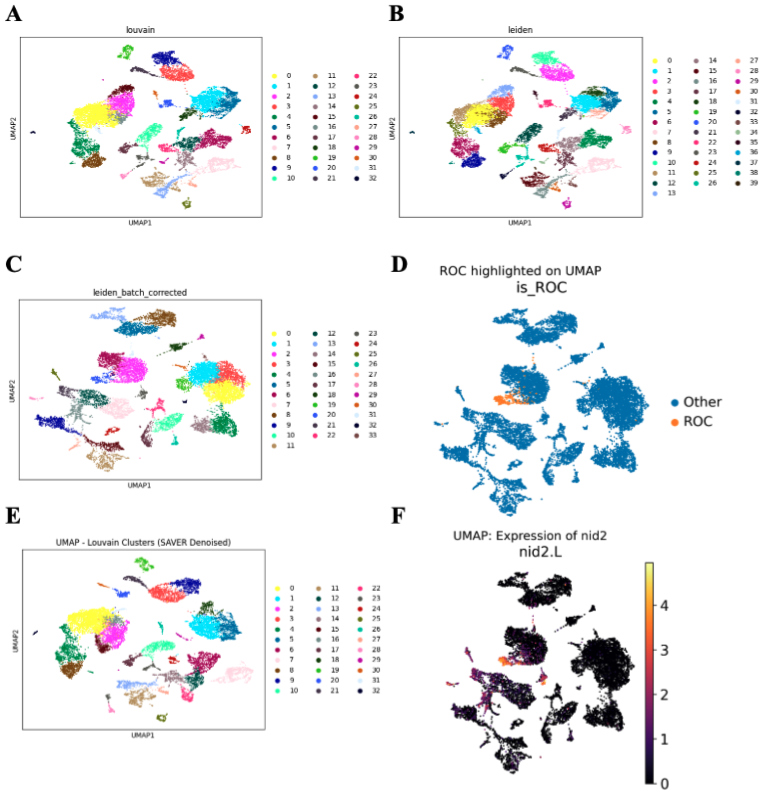
\includegraphics[width=0.8\textwidth]{figure1A.png}
    \caption{UMAP visualization colored by identified individual clusters (A) Louvain and (B) Leiden Clustering. (C)- Harmony Batch Corrected UMAP. (D)- ROC highlighted UMAP. (E)- SAVER Denoised UMAP. (F)- nid2 highlighted UMAP}
    \label{fig:umap}
\end{figure}

% ------------------------------------------------------------
\section{Conclusion}
In summary, we identified nid2 as the most persistent marker of the Regenerative Organizing Cell.  Among pre-processing methods, Harmony provided the most stable clustering structure, while diffusion-based denoising yielded the highest separation of cell states, and SAVER denoising yielded the most identified ROC marker genes, demonstrating its unique capability in recovering true biological data signal. These results support integrating pre-processing pipelines for robust and reliable single-cell identification of regenerative cell populations.

% ------------------------------------------------------------
\begin{thebibliography}{9}

\bibitem{paper1}
Jason Ye, [Code] JYY2142--Frog-Tail-MiniProject[Github Repo]: https://github.com/jasonye9/JYY2142--Frog-Tail-MiniProject/tree/main\\

\bibitem{paper2}
C. Aztekin\textit{et al.} Identification of a regeneration-organizing cell in the \textit{Xenopus} tail.\textit{Science}\textbf{364},653-658(2019).DOI:\href{https://doi.org/10.1126/science.aav9996}{10.1126/science.aav9996}

\bibitem{paper3}
Luecken, M.D., Gigante, S., Burkhardt, D.B. \textit{et al.} Defining and benchmarking open problems in single-cell analysis. \textit{Nat Biotechnol} 43, 1035–1040 (2025). https://doi.org/10.1038/s41587-025-02694-w

\bibitem{paper4}
Wolf, F. A., Angerer, P., \& Theis, F. J. (2018). \textit{SCANPY: large-scale single-cell gene expression data analysis.} Genome Biology, 19(1), 15.
https://doi.org/10.1186/s13059-017-1382-0

\bibitem{paper4}
Duò, A., Robinson, M. D., \& Soneson, C. (2018). \textit{A systematic performance evaluation of clustering methods for single-cell RNA-seq data.} F1000Research, 7, 1141.
https://doi.org/10.12688/f1000research.15666.1

\bibitem{paper4}
Korsunsky, I., Millard, N., Fan, J., Slowikowski, K., Zhang, F., Wei, K., ... \& Raychaudhuri, S. (2019). \textit{Fast, sensitive, and accurate integration of single-cell data with Harmony.} Nature Methods, 16(12), 1289–1296.
https://doi.org/10.1038/s41592-019-0619-0

\bibitem{paper4}
Huang, M., Wang, J., Torre, E., Dueck, H., Shaffer, S., Bonasio, R., Murray, J. I., Raj, A., Li, M., \& Zhang, N. R. (2018). \textit{SAVER: gene expression recovery for single-cell RNA sequencing.} Nature Methods, 15(7), 539–542.
https://doi.org/10.1038/s41592-018-0033-z

\bibitem{paper4}
Pullin, J., Chang, J., Gao, T., Zhang, H., Zhang, A. W., \& Campbell, K. R. (2024). \textit{A comparison of marker gene selection methods for single-cell data.} Briefings in Bioinformatics, 25(3), bbae103.
https://doi.org/10.1093/bib/bbae103

\bibitem{paper4}
Huang, M., Wang, J., Torre, E., Dueck, H., Shaffer, S., Bonasio, R., Murray, J. I., Raj, A., Li, M., \& Zhang, N. R. (2018). \textit{SAVER: gene expression recovery for single-cell RNA sequencing.} Nature Methods, 15(7), 539–542.
https://doi.org/10.1038/s41592-018-0033-z

\end{thebibliography}

\end{document}



